\documentclass[12pt]{article}
\usepackage{amsmath,amssymb,mathrsfs,fancyhdr,syntonly,lastpage,hyperref,enumitem,graphicx,subcaption, tikz}

\usepackage[thmmarks,thref]{ntheorem}

\theoremstyle{nonumberplain}
\theoremheaderfont{\itshape}
\theorembodyfont{\upshape}
\theoremseparator{.}
\theoremsymbol{\ensuremath{\square}}
\newtheorem{solution}{Solution}

\hypersetup{colorlinks=true,urlcolor=black}

\topmargin      -1.5cm   % read Lamport p.163
\oddsidemargin  -0.04cm  % read Lamport p.163
\evensidemargin -0.04cm  % same as oddsidemargin but for left-hand pages
\textwidth      16.59cm
\textheight     23.94cm
\parskip         7.2pt   % sets spacing between paragraphs
\parindent         0pt   % sets leading space for paragraphs
\pagestyle{empty}        % Uncomment if don't want page numbers
\pagestyle{fancyplain}


\usepackage{Sweave}
\begin{document}
\Sconcordance{concordance:RoughDraft.tex:RoughDraft.Rnw:%
1 25 1 1 0 93 1}

\lhead{05-30-2019}
\chead{CSAFE - Hough Grooves Document Process}
\rhead{Page \thepage\ of \pageref{LastPage}}

\section{Introduction}

\section{Methods}


In order to best identify the GEAs we first want to diminish noise in the image. This can be achieved by converting each scan into an image gradient, which signifies where there are directional changes in the color of the image. This approach unforunately loses most of the detail of the three dimensional scans, however, it better highlights the differences between LEAs and GEAs. Once an image gradient is obtained we select only edges we consider to be "strong", meaning they have a magnitude above the 99th percentile. Our reason for not fully carrying out a Canny Edge detection algorithm before using a Hough transform is that the Canny Edge algorithm increases processing time by about 35 seconds per image and actually highlights more striae and breakoff. 

\begin{figure}[!ht]
    \centering
    \begin{subfigure}{.5\textwidth}
      \centering
      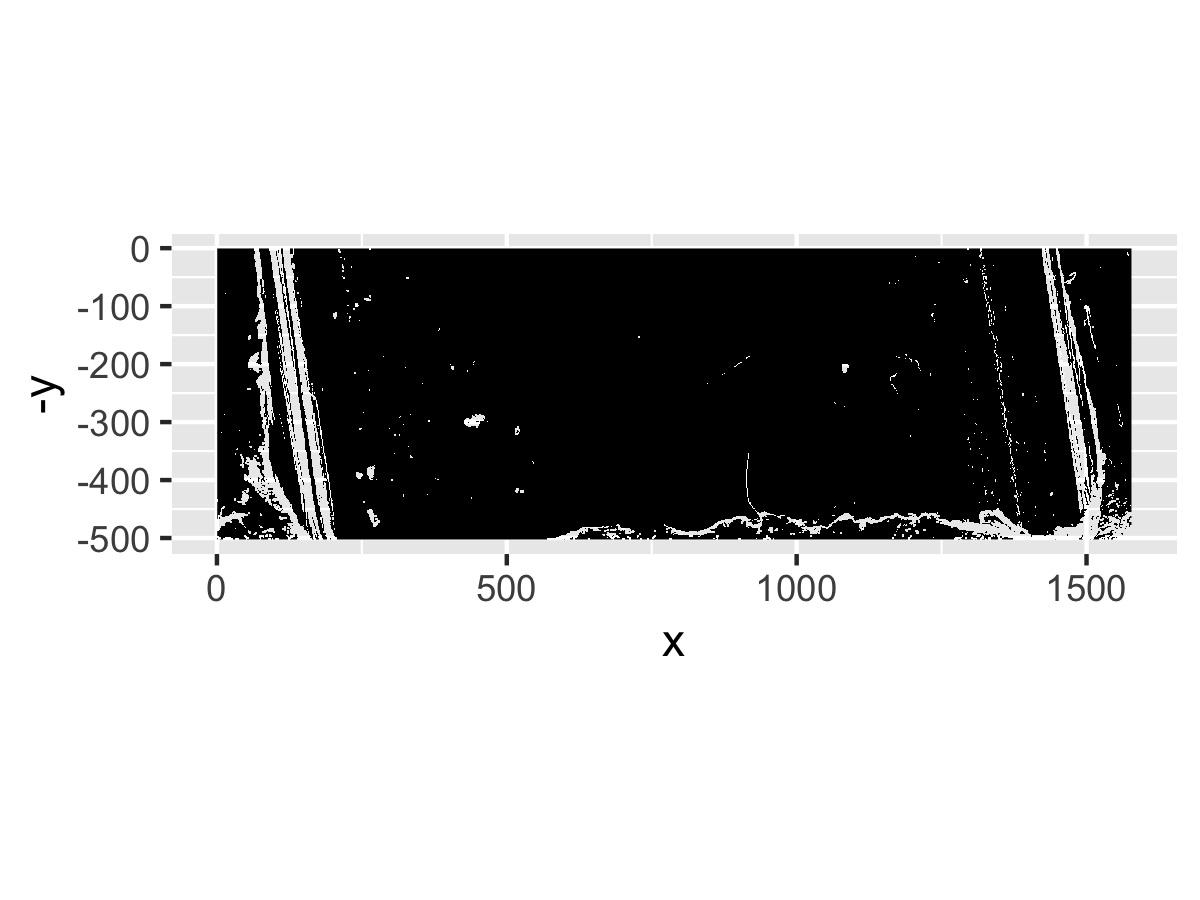
\includegraphics[width = .9\textwidth]{../images/Hamby252_Bullet1_Land3_Strong_edge.png}
      \caption{Edges with magnitudes in the 99th percentile}
      \label{fig: edge1}
      \end{subfigure}%
    \begin{subfigure}{.5\textwidth}
      \centering
      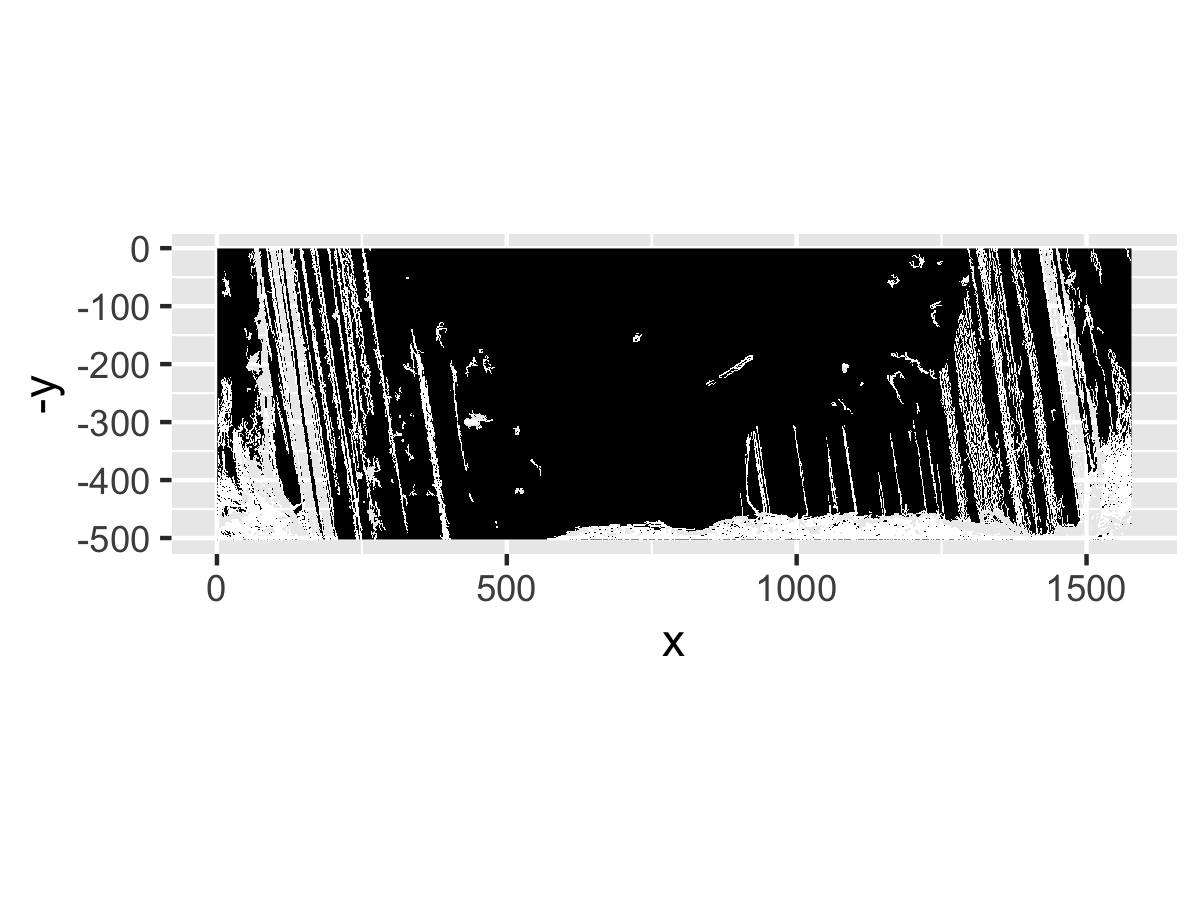
\includegraphics[width = .9\textwidth]{../images/Hamby252_Bullet1_Land3_Canny_Edge.png}
      \caption{Edges improved with Canny edge detection}
      \label{fig: edge2}
      \end{subfigure}
      \caption{Side-by-side comparison of Hamby 252 Bullet using both magnitude thresholding and Canny edge detection}
      \label{fig: canny}
\end{figure}

As shown in Figure \ref{fig: canny} the striae in the LEA are much more pronunced than in the image with only strong edges. We wish to focus on only detecting GEAs, so detecting an increased number of striae through Canny edge detection is not useful for our algorithm. Once we obtain the image gradient with only the strong edges we can then utilize our Hough transformation to obtain generally reasonable estimates of image boundaries. For the Hough transformation we utilize the function `` \texttt{hough\char`_lines}" from the imager package with the number of bins set to 100. While changing the number of bins does not seem to effect the processing time of the Hough transform, having a larger number of bins increases the number of extraneous detected lines in the image. For example in Figure \ref{fig: hough-compare}\subref{fig: hough1} we can see that the Hough transforms with 100 bins does a perfectly aedequate job of picking up the suspected grooves of the bullet. Therefore the extra detected lines in \ref{fig: hough-compare}\subref{fig: hough2} are not used in our analysis so we chose to limit our bin number as a result.

\begin{figure}[!ht]
    \centering
      \begin{subfigure}{.5\textwidth}
      \centering
      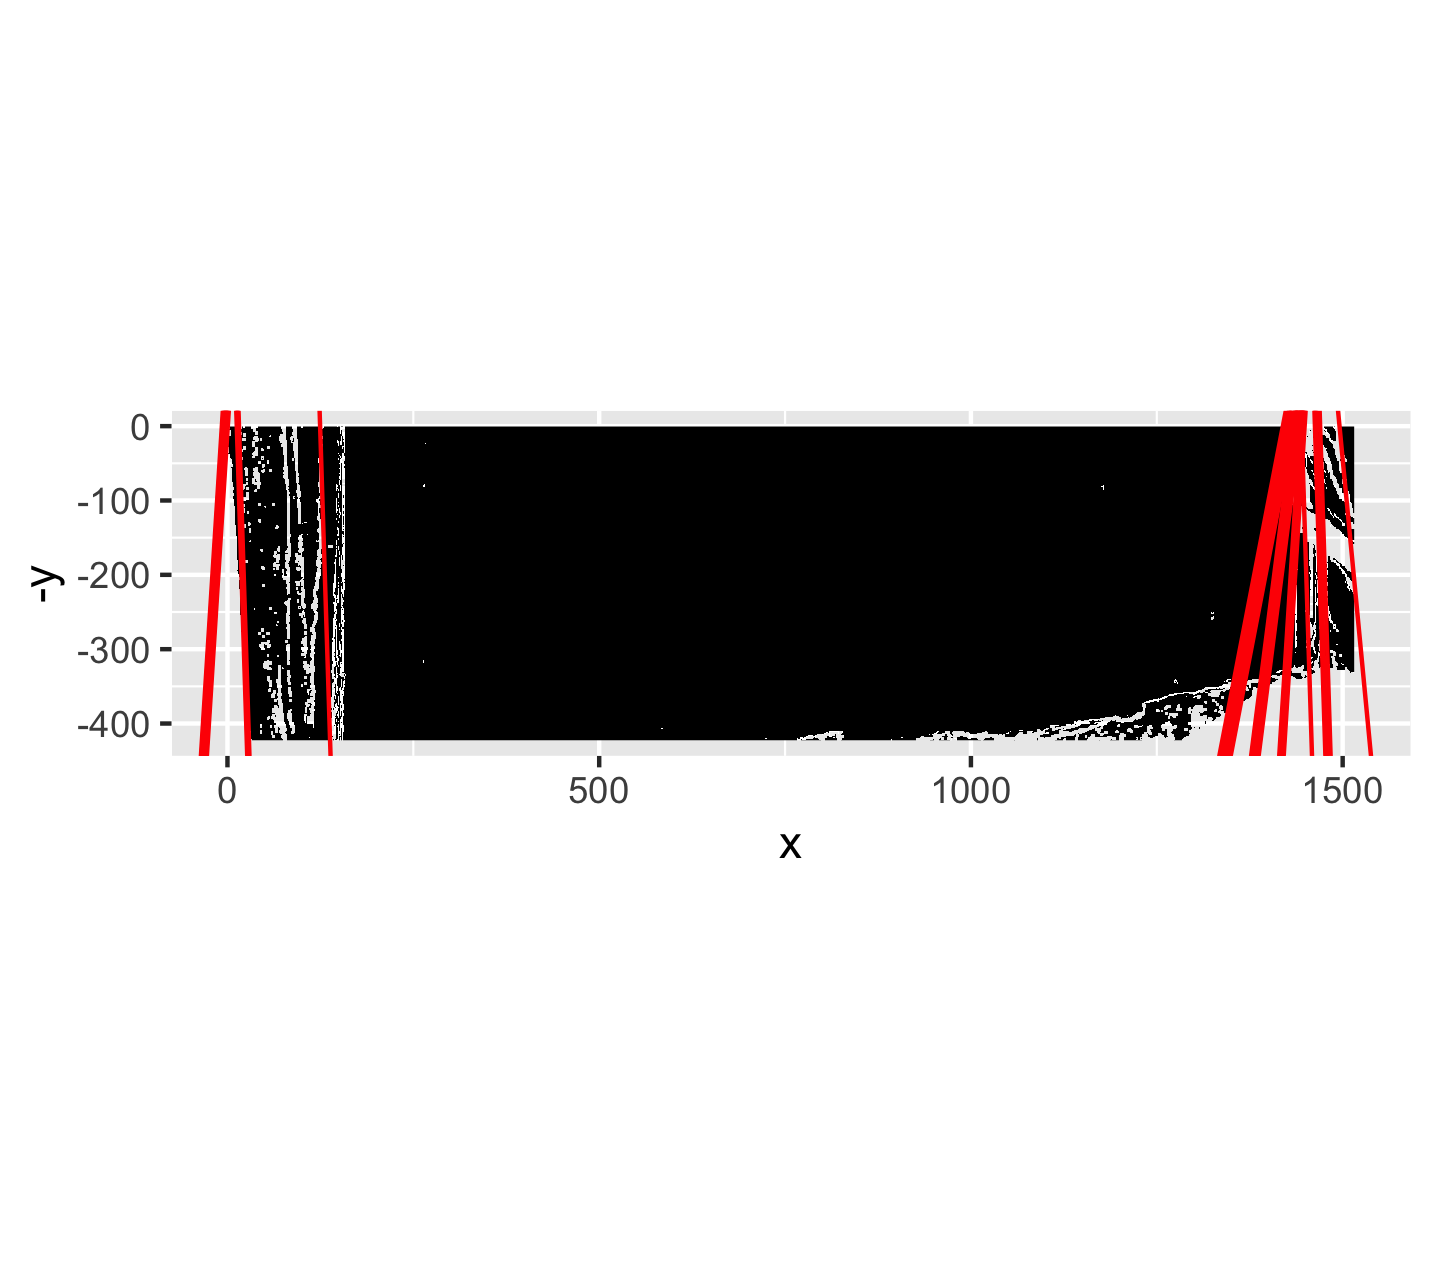
\includegraphics[width = .9\textwidth]{../images/Houston_BarrelF_Bullet1_Hough_Bin100}
      \caption{Hough Transform with 100 bins}
      \label{fig: hough1}
      \end{subfigure}%
    \begin{subfigure}{.5\textwidth}
      \centering
      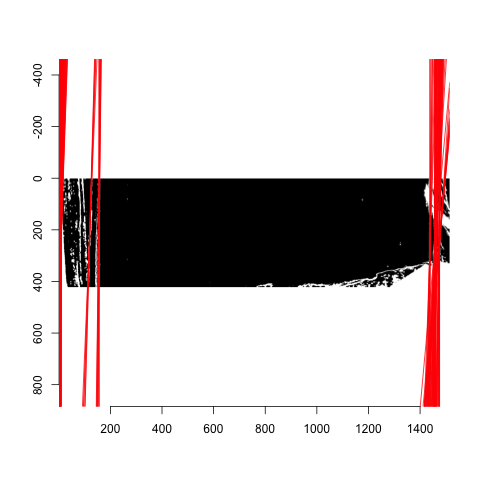
\includegraphics[width = .9\textwidth]{../images/Houston_BarrelF_Bullet1_Hough_Bin900}
      \caption{Hough Transform with 900 bins}
      \label{fig: hough2}
      \end{subfigure}
      \caption{Side-by-side comparison of Houston Barrel F Land 1 Hough Transformation. Hough lines are filtered by having scores in the 99.9th percentile, and having central angles less than $\frac{\pi}{4}$.}
      \label{fig: hough-compare}
\end{figure}

Once Hough lines are calculated we select only the lines that have scores greater than the $99.9^{th}$ percentile to try and ensure that we are dealing with only the strongest edges and do not accidentally pick up on any particularly strong striae on the LEAs. We also make the assumption that scans are oriented properly and as such, most Hough lines that correlate to the GEAs will be roughly vertical with some deviations in angle based on scanning technique. Therefore we select only the Hough lines that have angles from the positive x-axis less than $\frac{\pi}{4}$ and greater than $\frac{-\pi}{4}$. The parametrization outputted by `` \texttt{hough\char`_lines}" is of the form:

\begin{center}
$\rho = x \ cos(\theta) \ + \ y \ sin(\theta)$
\end{center}

Where $\rho$ represents the length of the normalized vector between the detected line and the origin of the image, and $\theta$ is the angle between the positive x-axis and the normalized vector. In Figure \ref{fig: parametrization} we see an example of how Hough transforms parametrize a line.

\begin{figure}[!ht]
  \begin{subfigure}{.5\textwidth}
    \centering
    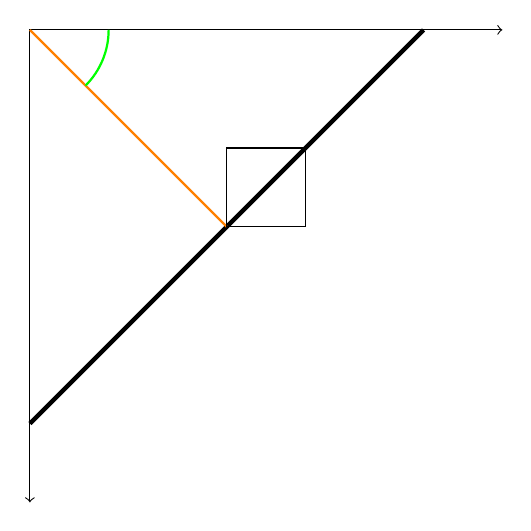
\begin{tikzpicture}
      \draw [<->] (0,-6) -- (0,0) -- (6,0);
      \draw [ultra thick] (0,-5) -- (5,0);
      \draw [orange, thick] (0,0) -- (2.5, -2.5);
      \draw [green, thick] (1,0) arc [radius = 1, start angle = 0, end angle = -45];
      \draw [black] (2.5, -2.5) rectangle (3.5,-1.5);
    \end{tikzpicture}
  \label{fig: tikz1}
  \end{subfigure}
  \begin{subfigure}{.5\textwidth}
    \centering
    \begin{tikzpicture}
      \draw [<->] (0,-6) -- (0,0) -- (6,0);
      \draw [ultra thick] (3,-6) -- (3,0);
      \draw [orange, thick] (0,0) -- (3,0);
    \end{tikzpicture}
    \label{fig: tikz2}
  \end{subfigure}
  \caption{Diagram of Hough transform parametrization oriented for image origin.}
  \label{fig: parametrization}
\end{figure}

We note that when $\theta$ is equal to 0, the x-intercept is given by $\rho$ however when $\theta$ is not 0 we utilize the above equation to find that the x-intercept is equivalent to $\frac{\rho}{\cos(\theta)}$. We then calculate the slope and the y-intercept in a similar fashion. To determine which Hough line is the boundary of each GEA we rely on the assumption that the middle two thirds of each bullet scan is often part of the LEA. Therefore, we find the x-intercept of the lower and upper one sixth of our bullet scan then compare these boundaries to each Hough Line. It is important to note at this point in the explanation that when we refer to $x$ and $y$, we are referring to the indices of the surface matrix of the x3p file rather than the specific microns of the land. With this in mind, we then find the x-intercept of each Hough line at both the top of the land (defined to be y = 0) and the bottom of the land (y = the number of rows of the x3p-surface matrix). Then each x-intercept for the tops and bottoms of the Hough lines are compared to the x-intercepts for the lower and upper one-sixth boundaries. The Hough x-intercept that is the smallest distance from the upper and lower one-sixth boundaries x-intercepts are selected for groove identification. We then calculate the equation of the line that connects these four sets of points. INSERT TIXZ DIAGRAM HERE

The output of the function get\textunderscore hough\textunderscore grooves is thus a list of two groove fits that extend across the entire height of the land. The functions for calculating each groove estimate are as follows:

\begin{align}
slope &= \frac{-(height \ of \ the \ image)}{(top.index - bottom.index)} \\
intercept &= ((- slope * top.index) - 1 ) * resolution
\end{align}

Where the resolution is the resolution of the x3p-file scan, obtained by using the bulletxtrctr command x3p\textunderscore get\textunderscore scale. 
\section{Results?}

In Figure \ref{fig: bestfit1} we show both the middle two thirds of the bullet land and the estimated best fit for the grooves based on our Hough transform.

\begin{figure}[!ht]
  \centering
  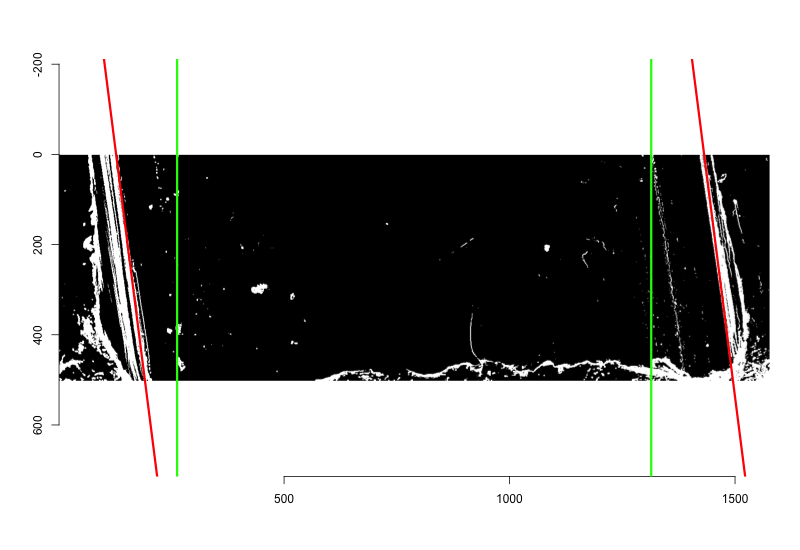
\includegraphics[width = .9\textwidth]{../images/Hamby_252_Bullet1_Land3_BestFit}
  \caption{Houstong Barrel F Bullet 1 middle two-thirds of the bullet land shown in green. Estimated Start of GEA shown in red}
  \label{fig: bestfit1}
\end{figure}

 

\end{document}
